\documentclass{../c-lecture}

\usepackage{algorithm2e}
\SetKwComment{Comment}{/* }{ */}

\subtitle{Algorithm Design}

\begin{document}

\begin{frame}
  \titlepage{}
\end{frame}

\begin{frame}
  \frametitle{What We Will Learn}
  \begin{itemize}
    \item Sample algorithms to practice problem solving steps
    \item Input \& Output analysis
    \item Algorithm design
    \begin{itemize}
      \item Pseudo-code
    \end{itemize}
  \end{itemize}
\end{frame}

\begin{frame}
  \frametitle{Average}
  \begin{algorithm}[H]
  \KwData{$x_1, x_2, x_3$}
  \KwResult{$avg(x_1, x_2, x_3)$}
  $sum \gets x_1 + x_2 + x_3$\;
  $avg \gets sum / 3$\;
  print ``average = '' $avg$ \;
  \end{algorithm}
\end{frame}

\begin{frame}
  \frametitle{Odd-Even-1}
  \begin{algorithm}[H]
  \KwData{$n \in \mathbb{Z}$}
  \KwResult{$n$ is even or odd}
  $r \gets n \% 2$\;
  \eIf{$r == 0$}{%
      print $n$ ``is even''\;
    }{%
      print $n$ ``is odd''\;
    }
  \end{algorithm}
\end{frame}

\begin{frame}
  \frametitle{Odd-Even-2}
  \begin{algorithm}[H]
  \KwData{$n \in \mathbb{Z}$}
  \KwResult{$n$ is even or odd}
  \If{n < 0}{%
    $n \gets -1 * n$\;
  }
  \While{$n \geq 0$}{%
    $n \gets n - 2$\;
  }
  \eIf{$n == 0$}{%
      print $n$ ``is even''\;
    }{%
      print $n$ ``is odd''\;
    }
  \end{algorithm}
\end{frame}

\begin{frame}
  \frametitle{Odd-Even-3}
  \begin{algorithm}[H]
  \KwData{$n \in \mathbb{Z}$}
  \KwResult{$n$ is even or odd}
  $r \gets n \% 2$\;
  \While{$n \geq 0$ or $n \leq -1$}{%
    $n \gets n - sign(n) * 2$\;
  }
  \eIf{$n == 0$}{%
      print $n$ ``is even''\;
    }{%
      print $n$ ``is odd''\;
    }
  \end{algorithm}
\end{frame}

\begin{frame}
  \frametitle{Count Odd-Even}
  \begin{block}{}
    The algorithm read array of numbers that are ending with 0 then count even
    and odd numbers.
  \end{block}
\end{frame}

\begin{frame}
  \frametitle{Count Odd-Even}
  \begin{algorithm}[H]
  \KwData{$\forall n \in \mathbb{Z}$}
  \KwResult{number of even and odd numbers}
  $even\_cnt \gets 0$\;
  $odd\_cnt \gets 0$\;
  read $n$\;
  \While{$n \neq 0$}{%
    $r \gets n \% 2$\;
    \eIf{$r == 0$}{%
      $even\_cnt \gets even\_cnt + 1$\;
    }{%
      $odd\_cnt \gets odd\_cnt + 1$\;
    }
    read $n$\;
  }
  print ``Odd = '' $odd\_cnt$ ``Even = '' $even\_cnt$\;
  \end{algorithm}
\end{frame}

\begin{frame}
  \frametitle{Digit-Sum}
  \begin{algorithm}[H]
  \KwData{$n \in \mathbb{Z} \geq 0$}
  \KwResult{sum of digits}
  $sum \gets 0$\;
  $m \gets n$\;
  \While{$n \neq 0$}{%
    $d \gets n \% 10$\;
    $sum \gets sum + d$\;
    $n \gets n - d$\;
    $n \gets n / 10$\;
  }
  print ``sum of digits of'' $m$ `` = '' $sum$\;
  \end{algorithm}
\end{frame}

\begin{frame}
  \frametitle{Base-8}
  \begin{algorithm}[H]
  \KwData{$n \in \mathbb{Z} \geq 0$}
  \KwResult{$n$ in base-8}
  $i \gets 0$\;
  \While{$n \neq 0$}{%
    $x[i] \gets n \% 8$\;
    $n \gets \lfloor n / 8 \rfloor$\;
    $i \gets i + 1$\;
  }
  \While{$i \geq 0$}{%
    $i \gets i - 1$\;
    print $x[i]$
  }
  \end{algorithm}
\end{frame}

\begin{frame}
  \frametitle{Factorial-1}
  \begin{algorithm}[H]
  \KwData{$n \in \mathbb{Z} \geq 0$}
  \KwResult{$ result = n! $}
  $i \gets 1$\;
  $result \gets 1$\;
  \While{$i \leq n$}{%
    $result \gets i * result$\;
    $i \gets i + 1$\;
  }
  \end{algorithm}
\end{frame}

\begin{frame}
  \frametitle{Factorial-2}
  \begin{algorithm}[H]
  \KwData{$n \in \mathbb{Z} \geq 0$}
  \KwResult{$ result = n! $}
  $result \gets 1$\;
  \While{$n \geq 0$}{%
    $result \gets n * result$\;
    $n \gets n - 1$\;
  }
  \end{algorithm}
\end{frame}

\begin{frame}
  \frametitle{$factorial\_recursive(n)$}
  \begin{algorithm}[H]
  \KwData{$n \in \mathbb{Z} \geq 0$}
  \KwResult{$ factorial\_recursive(n) = n! $}
  \eIf{n == 1}{%
    return 1\;
  }{%
    return $n * factorial\_recursive(n - 1)$\;
  }
  \end{algorithm}
\end{frame}

\begin{frame}
  \frametitle{$sort(X, start, end)$}
  \begin{algorithm}[H]
  \KwData{$X = \{x | x \in \mathbb{Z}\}$}
  \KwResult{sorted $X$}
  \While{$start \neq end$}{%
    $j \gets find\_\min(X, start, end)$\; \Comment*[r]{find index of minimum element from $start$ to $end$}
    $swap(X[j], X[start])$\;
    $start \gets start + 1$\;
  }
  \end{algorithm}
\end{frame}

\begin{frame}
  \frametitle{$find\_\min(X, start, end)$}
  \begin{algorithm}[H]
  \KwData{$X = \{x | x \in \mathbb{Z}\}$}
  \KwResult{$index$ = index of minimum element from $X$}
  $i \gets start$\;
  $index \gets i$\;
  \While{$i \leq end$}{%
    \If{$X[i] < X[index]$}{%
      $index \gets i$\;
    }
    $i \gets i + 1$\;
  }
  \end{algorithm}
\end{frame}

\begin{frame}
  \frametitle{$swap(X, j, i)$}
  \begin{algorithm}[H]
  \KwData{$X = \{x | x \in \mathbb{Z}\}$}
  \KwResult{}
  $tmp \gets X[j]$\;
  $X[j] \gets X[i]$\;
  $X[i] \gets temp$\;
  \end{algorithm}
\end{frame}

\begin{frame}
  \frametitle{$reverse(A, start, end)$}
  \begin{algorithm}[H]
  \KwData{$A = \{a | a \in \mathbb{Z}\}$}
  \KwResult{A in a reverse order}
  \eIf{$start \geq end$}{%
    return\;
  }{%
    $swap(A, start, end)$\;
    $reverse(A, start + 1, end - 1)$\;
  }
  \end{algorithm}
\end{frame}

\begin{frame}
  \frametitle{Summary}
  \begin{itemize}
    \item There are more than one algorithm for a problem
    \begin{itemize}
      \item Efficiency, Complexity, Clarity, \ldots
    \end{itemize}
    \item Algorithm (Programming Language) building blocks
    \begin{itemize}
      \item Input / Output (Lecture 5)
      \item Calculations (Lecture 4)
      \item Decision Making (Lecture 6)
      \item Repeating (Lecture 7)
      \item Modular Programming (Lecture 8)
      \item Arrays + Memory Management (Lectures 9 + 10)
      \item Others (Files, …) (Lecture 11 + 12)
    \end{itemize}
  \end{itemize}
\end{frame}

\begin{frame}
  \frametitle{Legends}
  \begin{figure}
    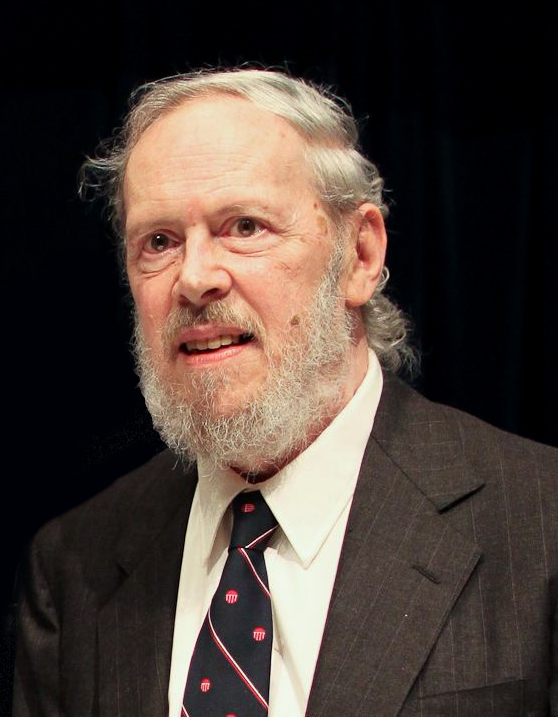
\includegraphics[height=.75\textheight]{./img/dennis.jpg}
  \end{figure}
  \pause%
  \centering
  \color{Violet} Dennis Ritchie
\end{frame}

\end{document}
